\documentclass[letterpaper]{article}
\usepackage[utf8]{inputenc}
\usepackage[T1]{fontenc}
\usepackage[activeacute,spanish]{babel}
\usepackage[vmargin=4cm,tmargin=3cm,hmargin=2cm,letterpaper]{geometry}%
\usepackage{helvet}
\usepackage{amsmath,amsfonts,amssymb}
\usepackage{graphicx}
\usepackage{color}
\usepackage{xcolor}
\usepackage{verbatim}
\usepackage{tabls}
\usepackage{lastpage}
\usepackage{fancyhdr}
\usepackage{url}
\usepackage{listings}
%%%%%%%%%%%%%%%%%%%%%%%%%%%%%%%%%%%%%%%%%%%%%%%%%%%%%%%%%%%%%%%%%%%%%%%%%%%%%%%%%%%%%%%
\usepackage{tikz}
\usepackage{pgf}
\usepackage{pgffor}
\usepgfmodule{plot}
\usepackage{wrapfig}
\usetikzlibrary{arrows,decorations,snakes,backgrounds,fit,calc,through,scopes,positioning,automata,chains,er,fadings,calendar,matrix,mindmap,folding,patterns,petri,plothandlers,plotmarks,shadows,shapes,shapes.arrows,topaths,trees}

\lstset{% general command to set parameter(s)
%   basicstyle=\small,
  % print whole listing small
%   keywordstyle=\color{black}\bfseries\underbar,
  % underlined bold black keywords
%   identifierstyle=,
  % nothing happens
%   commentstyle=\color{white}, % white comments
%   stringstyle=\ttfamily,
  % typewriter type for strings
  showstringspaces=false}
  % no special string spaces

\pagestyle{fancy}
\color{black}
\fancyhead{}
\renewcommand{\headrule}{\hrule\vspace*{0.5mm}\rule{\linewidth}{0.8mm}}
\renewcommand{\familydefault}{\sfdefault}

\graphicspath{{./images/}}
\lhead{
\includegraphics[width=2cm]{logoucr.png}}
\rhead{
\includegraphics[width=3cm]{eie-text-gray-6x3cm.png}}
\chead{UNIVERSIDAD DE COSTA RICA\\FACULTAD DE INGENIERÍA\\ESCUELA DE INGENIERÍA ELÉCTRICA\\\textbf{ESTRUCTURAS ABSTRACTAS DE DATOS Y\\ ALGORITMOS PARA INGENIERÍA}\\IE-0217\\I CICLO 2014\\PROYECTO ESTRUCTURAS DE DATOS Y ALGORITMOS}

\lfoot{}%
\cfoot{}%
%\cfoot{\thepage\ de \pageref{LastPage}}%
\rfoot{}%

%%%%%%%%%%%%%%%%%%%%%%%%%%%%%%%%%%%%%%%%%%%%%%%%%%%%%%%%%%%%%%%%%%%%%%%%%%%%%%%%%%%%%%%%%%%%%%%%%%%%%%%%%%%%%%%
\newcommand{\uic}{black} %user-input color
%%%%%%%%%%%%%%%%%%%%%%%%%%%%%%%%%%%%%%%%%%%%%%%%%%%%%%%%%%%%%%%%%%%%%%%%%%%%%%%%%%%%%%%%%%%%%%%%%%%%%%%%%%%%%%%%%%
\newcommand{\uim}{} %user-input marker
%%%%%%%%%%%%%%%%%%%%%%%%%%%%%%%%%%%%%%%%%%%%%%%%%%%%%%%%%%%%%%%%%%%%%%%%%%%%%%%%%%%%%%%%%%%%%%%%%%%%%%%%%%%%%%%%%%
\newcommand{\userinput}[1]{\textcolor{\uic}{\uim#1\uim}}


%%%%%%%%%%%%%%%%%%%%%%%%%%%%%%%%%%%%%%%%%%%%%%%%%%%%%%%%%%%%%%%%%%%%%%%%%%%%%%%%%%%%%%%%%%%%%%%%%%%%%%%%%%%%%%%%%%
\begin{document}\vspace*{2cm}
%%%%%%%%%%%%%%%%%%%%%%%%%%%%%%%%%%%%%%%%%%%%%%%%%%%%%%%%%%%%%%%%%%%%%%%%%%%%%%%%%%%%%%%%%%%%%%%%%%%%%%%%%%%%%%%%%%

%%%%%%%%%%%%%%%%%%%%%%%%%%%%%%%%%%%%%%%%%%%%%%%%%%%%%%%%%%%%%%%%%%%%%%%%%%%%%%%%%%%%%%%%%%%%%%%%%%%%%%%%%%%%%%%%%%
\begin{center}
\Huge
\userinput{Análisis de complejidad y correctitud de los algoritmos de compresión y descompresión del sistema de empaquetado Ilsh(Implementación LZW-Hash)}
\vspace*{1cm}
\end{center}

\noindent
\small\baselineskip=14pt
\textbf{Estudiantes:}\\
\userinput{Willy Villalobos Marrero B17170}\\
\userinput{Daniel Méndez Zeledón A83911}\\
\userinput{Javier Acosta Villalobos A80056}\\


%%%%%%%%%%%%%%%%%%%%%%%%%%%%%%%%%%%%%%%%%%%%%%%%%%%%%%%%%%%%%%%%%%%%%%%%%%%%%%%%%%%%%%%%%%%%%%%%%%%%%%%%%%%%%%%%%%
\section{Introducción}

A partir de la segunda mitad del curso y como complemento de la programación en C++, se aprendió a realizar análisis que permiten determinar si los algoritmos son óptimos, que tan rápidos son y como mejorarlos. Como parte del proyecto, se va a tomar el algoritmo descrito por uno de los presentes en este proyecto como parte del curso y se le harán mejoras en caso de ser necesario, ademas de analizar su complejidad y su correctitud. El algoritmo que se va a analizar es el LZW utilizando tabla Hash, el cual genera un gran aporte a la compresión de los archivos.\\

Es importante destacar que el LZW ya por si solo es un excelente compresor, ya que presenta la característica de que no necesita guardar una tabla de compresión para que el descompresor entienda como está codificado el archivo, sino que, como usalos caracteres del sistema, que son los ASCII, ya de antemano el descompresor sabe al menos cuales son los valores iniciales de la tabla de compresión, para luego, de forma automática, se cree la tabla para continuar con la descompresión.\\

A su vez, el código se pasa a través de un hash que luego será ordenado en una tabla hash. Un hash es un algoritmo que permite modificar un código para que sea casi unívoco a un registro, archivo o documento. Una tabla hash o mapa hash es una estructura de datos que asocia llaves o claves con valores. Una tabla hash se puede ver como un conjunto de entradas. Cada una de estas entradas tiene asociada una clave única, y por lo tanto, diferentes entradas de una misma tabla tendrán diferentes claves. Esto implica, que una clave identifica de manera unívoca a una entrada de una tabla hash.\\

Todo esto implica una reducción en el tamaño del archivo original que nos va a permitir comprimir eficazmente el archivo, en nuestro caso de texto, haciendo que nuestro proyecto tenga validéz.\\

También, como parte del aporte al trabajo previo, se creará el algoritmo que descomprima los archivos de formato ilsh creados por el compresor y también se tratará de utilizar la teoría para hacer que éste sea lo más eficiente posible. De igual manera se le harán las respectivas pruebas de complejidad y correctitud paso por paso para así idenficar fallas del código como tal y las posibles mejoras a éstos.\\
%%%%%%%%%%%%%%%%%%%%%%%%%%%%%%%%%%%%%%%%%%%%%%%%%%%%%%%%%%%%%%%%%%%%%%%%%%%%%%%%%%%%%%%%%%%%%%%%%%%%%%%%%%%%%%%%%%
\section{Objetivos}
\subsection{Objetivo General}

Analizar el algoritmo para la implementacion del LZW con tabla Hash con el fin de obtener su rendimiento a partir del análisis de correctitud y complejidad aprendidos en el curso para determinar si existe mejoras frente a otros compresores de archivos.

\subsection{Objetivos Específicos}

\begin{itemize}

\item Analizar la complejidad del algoritmo de compresión de LZW con tabla Hash para determinar el desempeño del algorimto, utilizando un análisis línea a línea de la cantidad de operaciones que hace éste.
\item Realizar un análisis de correctitud con el fin de demostrar que el algoritmo es correcto, utilizando los invariantes de lazo que se puedan determinar para tal demostración.
\item Crear el algoritmo para el descompresor que no se había tenido listo y a su vez analizar su complejidad y correctitud de la misma manera que para el compresor, de las formas previamente descritas.
\item Crear los esquemas del modelo de ejecución del algoritmo con el fin de tener una mejor representación del algoritmo y así mejorar su documentación.\\

\end{itemize}


%%%%%%%%%%%%%%%%%%%%%%%%%%%%%%%%%%%%%%%%%%%%%%%%%%%%%%%%%%%%%%%%%%%%%%%%%%%%%%%%%%%%%%%%%%%%%%%%%%%%%%%%%%%%%%%%%%
\section{Descripción general de la implementación del LZW con tabla Hash}

El método de compresión LZW permite la compresión de datos de manera tal que no es necesaria un paso de la tabla de codificación dentro del archivo ni tampoco analiza doblemente el archivo para verificar la codificación, esto garantiza que el método es lo más rápido posible a su vez de que envía solamente los códigos necesarios al descompresor para analizar su codificación y descomprimirlo.\\

A su vez, el uso de tabla hash como método de organización de los códigos permite un mejoramiento en el rendimiento del compresor, aunque dura un poco más, pero genera códigos unívocos que permite la seguridad del archivo así como la seguridad de que la descompresión será completamente correcta.\\

Antes de entrar en discusión en el código y el análisis de éste, se van a mencionar por encima qué son las tablas hash y cómo funcionan, a su vez de como trabaja el algoritmo LZW implementados ambos para generar un mejor compresor.\\

\subsection{LZW}

LZW (Lempel-Ziv-Welch) es un algoritmo de compresión sin pérdida desarrollado por Terry Welch en 1984 como una versión mejorada del algoritmo LZ78 desarrollado por Abraham Lempel y Jacob Ziv.\\

El método LZW permite crear sobre la marcha, de manera automática y en una única pasada un diccionario de cadenas que se encuentren dentro del texto a comprimir mientras al mismo tiempo se procede a su codificación. Dicho diccionario no es transmitido con el texto comprimido, puesto que el descompresor puede reconstruirlo usando la misma lógica con que lo hace el compresor y, si está codificado correctamente, tendrá exactamente las mismas cadenas que el diccionario del compresor tenía.\\

El diccionario comienza pre-cargado con 256 entradas, una para cada carácter (byte) posible más un código predefinido para indicar el fin de archivo. A esta tabla se le van agregando sucesivos códigos numéricos por cada nuevo grupo de caracteres en orden úncio.\\

Es en este detalle donde se encuentra la brillantez del método: al armar el diccionario sobre la marcha se evita hacer dos pasadas sobre el texto, una analizando y la otra codificando y dado que la regla de armado del diccionario es tan simple, el descompresor puede reconstruirlo a partir del texto comprimido mientras lo lee, evitando así incluir el diccionario dentro del texto comprimido.\\

Las entradas del diccionario pueden representar secuencias de caracteres simples o secuencias de códigos de tal forma que un código puede representar dos caracteres o puede representar secuencias de otros códigos previamente cargados que a su vez representen, cada uno de ellos, otros códigos o caracteres simples, o sea que un código puede representar desde uno a un número indeterminado de caracteres. Los caracteres básicos que usa el compresor son 256 de 8 bits,que equivalen al códico ASCII.\\

Cada vez que se lee un nuevo carácter se revisa el diccionario para ver si forma parte de alguna entrada previa. Todos los caracteres están inicialmente predefinidos en el diccionario así que siempre habrá al menos una coincidencia, sin embargo, lo que se busca es la cadena más larga posible. Si el carácter leído no forma parte de más de una cadena más larga, entonces se crea una nueva entradaen la tabla con esta nueva cadena encontrada, tomando el siguiente código a disposicion. Si el carácter leído sí forma parte de más de una cadena del diccionario, se lee un nuevo carácter para ver si la secuencia formada por el carácter previo y el nuevo es alguna de las encontradas en el diccionario. En tanto los caracteres sucesivos que se vayan leyendo ofrezcan más de una entrada posible en el diccionario, se siguen leyendo caracteres. Cuando la cadena sólo tiene una entrada en el diccionario, entonces se emite el código correspondiente a esa entrada y se incorpora al diccionario una nueva entrada que representa el último código emitido y el nuevo.\\

El algoritmo tiene un límite de códigos de 16 bits, esto quiere decir que un diccionario nunca podrá contener más de 65536 entradas, cada una de ellas de 2 códigos de 16 bits, o sea cuatro bytes por entrada. El diccionario, entonces, se arma como una tabla donde el código es el índice y las cadenas que representa son las entradas de esta tabla. Adviértase que el código en si no se almacena en la tabla sino que es el índice de la misma por lo cual no se almacena sino que se calcula por la posición en la tabla. En total, una tabla llena ocupa 65536 entradas de 4 bytes cada una, o sea 262144 caracteres (256 kbytes) lo que es absurdamente poco para los ordenadores actuales.\\

\subsection{Tabla Hash}

El hash es un método o función para generar llaves o claves que representan de manera casi unívoca a un archivo, registro o incluso un documento; también se puede resumir o identificar un dato a través de la probabilidad, utilizando una función hash o algoritmo hash. Dicho de otra manera, una tabla hash es un contendor asociativo que permite un almacenamiento y posterior recuperación eficiente de elementos.\\

Algoritmo que se utiliza para generar un valor de hash para algún dato, como por ejemplo claves. Un algoritmo de hash hace que los cambios que se produzcan en los datos de entrada provoquen cambios en los bits del hash. Gracias a esto, los hash permiten detectar si un dato ha sido modificado.\\

Una tabla hash o mapa hash es una estructura de datos que asocia llaves o claves con valores. La operación principal que soporta de manera eficiente es la búsqueda: permite el acceso a los elementos almacenados a partir de una clave generada. Funciona transformando la clave con una funcion hash en un hash, un número que la tabla hash utiliza para localizar el valor deseado. Más a fondo, una tabla hash se puede ver como un conjunto de entradas. Cada una de estas entradas tiene asociada una clave única, y por lo tanto, diferentes entradas de una misma tabla tendrán diferentes claves. Esto implica, que una clave identifica de manera unívoca a una entrada de una tabla hash.\\

Por lo lado, las entradas de las tablas hash están compuestas por dos componentes, la propia clave y la información que se almacena en dicha entrada. Si el número de claves almacenadas en la tabla es pequeño en comparación con el número total de claves posibles, la estructura tabla de hash resulta una forma eficiente de implementación.\\

La estructura de las tablas hash es lo que les confiere su gran potencial, ya que hace de ellas unas estructuras extrema damente eficientes a la hora de recuperar información almacenada. Para almacenar la informaci[on en la tabla hash, se la misma funcion hash, por lo tanto, el tiempo medio de recuperación de información es constante, es decir, no depende del tamaño de la tabla ni del número de elementos almacenados en la misma.\\

\pagebreak

%%%%%%%%%%%%%%%%%%%%%%%%%%%%%%%%%%%%%%%%%%%%%%%%%%%%%%%%%%%%%%%%%%%%%%%%%%%%%%%%%%%%%%%%%%%%%%%%%%%%%%%%%%%%%%%%%%
\section{Diagramas de flujo de los algoritmos de compresión y descompresión}
Como parte del aporte que se le hizo al trabajo anterior, se hicieron los diagramas de flujo tanto para el compresor como para el descompresor. Permite visualizar mejor el funcionamiento de los dos algoritmos y demostrar el desarrollo del código implementado. A continuación se muestran los diagramas.

\subsection{Diagrama del compresor}

\begin{figure}[h!]
	\centering
	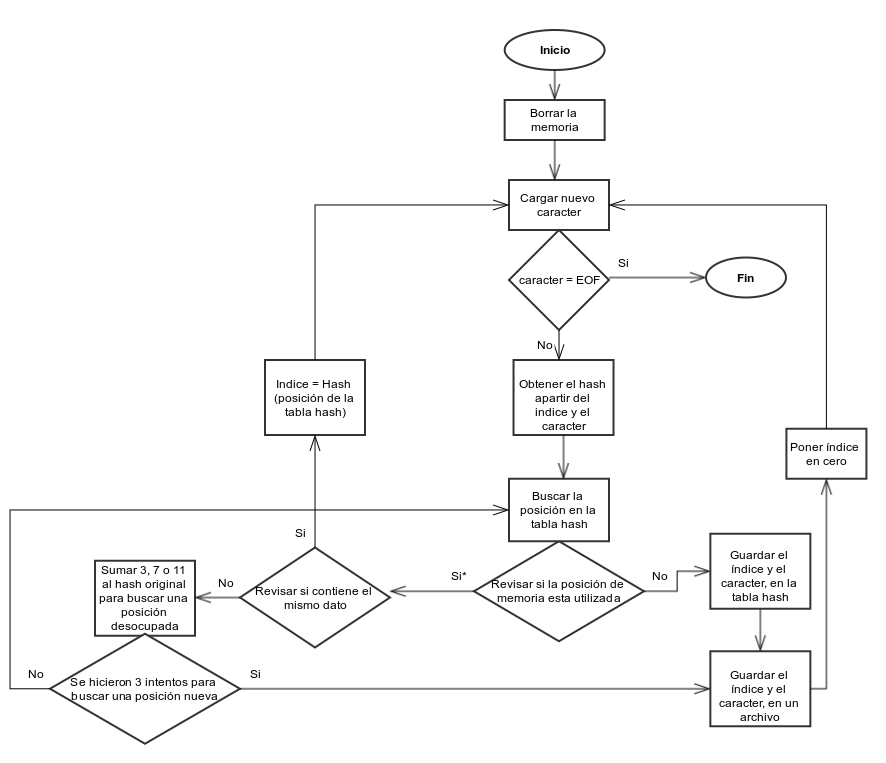
\includegraphics[width=0.99\textwidth]{compresorpng.png}
	\label{fig2}
	\caption{Diagrama de flujos del compresor}
\end{figure}

\pagebreak

\subsection{Diagrama del descompresor}


\begin{figure}[h!]
	\centering
	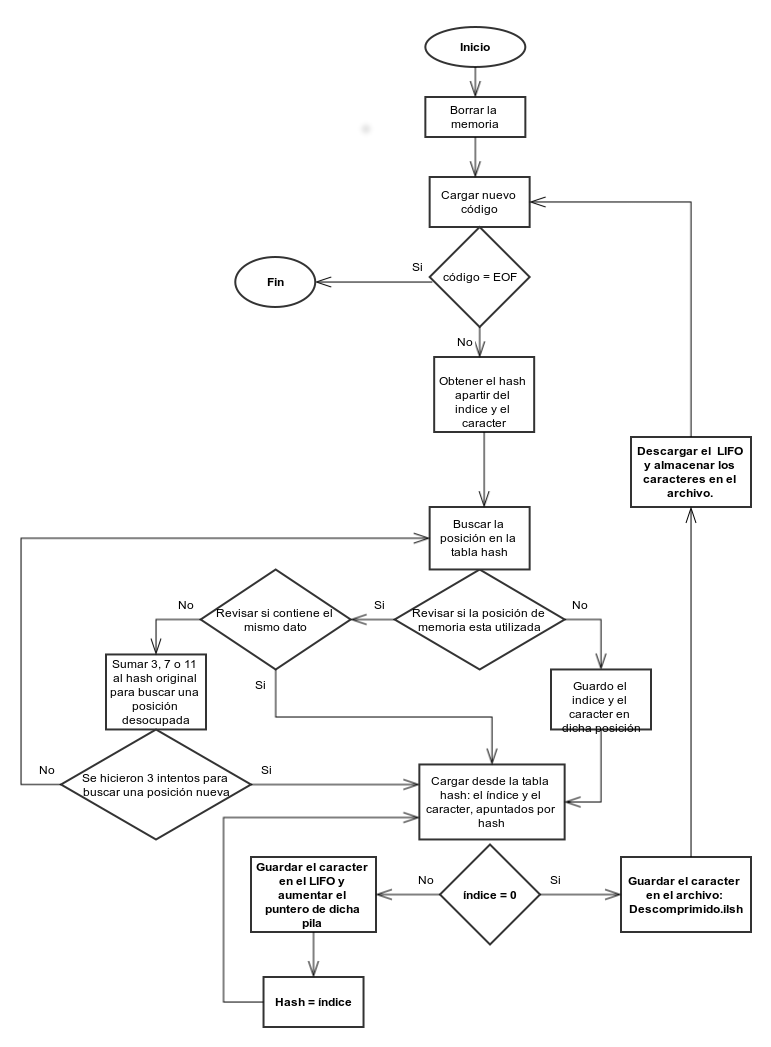
\includegraphics[width=0.75\textwidth]{descompresor.png}
	\label{fig2}
	\caption{Diagrama de flujos del descompresor}
\end{figure}


\pagebreak

%%%%%%%%%%%%%%%%%%%%%%%%%%%%%%%%%%%%%%%%%%%%%%%%%%%%%%%%%%%%%%%%%%%%%%%%%%%%%%%%%%%%%%%%%%%%%%%%%%%%%%%%%%%%%%%%%
\section{Análisis del algoritmo de compresión Ilsh}


\subsection{Análisis de complejidad}

A continuación se analiza línea por línea la cantidad de operaciones elementales que hace el algoritmo de compresión, esto para que al final nos de el orden del polinomio que sigue el algoritmo, lo que se denomina la complejidad del algoritmo. Con ésto podremos determinar las funciones asintóticas por arriba y por abajo que representan el máximo tiempo que dura el algoritmo.\\



\begin{tabular}{|l|c|c|c|}
\hline 
Línea de código & Operation Count & Worst Case & Best Case \\ 
\hline
int main() & 1 & 1 & 1 \\
\hline 
\hspace{0.5cm} char parte\_{alta}, parte\_{baja}; & 2 & 2 & 2 \\ 
\hline 
\hspace{0.5cm} int caracter\_{guardado}, indice\_{guardado}; & 2 & 2 & 2 \\ 
\hline 
\hspace{0.5cm} int Numero = 0, numero2 = 0; & 4 & 4 & 4 \\ 
\hline 
\hspace{0.5cm} int tabla\_{hash} [65536]; & 2 & 2 & 2 \\ 
\hline 
\hspace{0.5cm} for(int i=0;i$<$65536;i++) & 3n & 3n & 3 \\ 
\hline
\hspace{1cm} tabla\_hash[i]=0; & • & • & • \\ 
\hline
\hspace{0.5cm} FILE *pFile;& 1 & 1 & 1 \\ 
\hline 
\hspace{0.5cm} FILE *pFile2; & 1 & 1 & 1 \\ 
\hline 
\hspace{0.5cm} pFile = fopen (''cars\_0110.jpg'' , ''r''); & 1 & 1 & 1 \\ 
\hline 
\hspace{0.5cm} pFile2 = fopen(''Comprimido.ilsh'',''w''); & 1 & 1 & 1 \\ 
\hline 
\hspace{0.5cm} if (pFile == NULL \&\& pFile2 == NULL) perror (''Error opening file''); & 4 & 4 & 4 \\
\hline  
\hspace{0.5cm} else & 1 & 1 & 1 \\ 
\hline
\hspace{1cm} int indice = 0; & 2 & 2 & 2 \\ 
\hline
\hspace{1cm} unsigned char c; & 1 & 1 & 1 \\ 
\hline
\hspace{1cm} while(feof(pFile) == 0) & n & n & 1 \\ 
\hline
\hspace{1.5cm} c = fgetc (pFile); & 1 & 1 & 1 \\ 
\hline
\hspace{1.5cm} int caracter = c; & 2 & 2 & 2 \\ 
\hline
\hspace{1.5cm} int mov\_choque = 3; & 2 & 2 & 2 \\ 
\hline
\hspace{1.5cm} int trasl\_caracter = caracter\textless\textless 8; & 3 & 3 & 3 \\ 
\hline
\hspace{1.5cm} int hash = indice \^{} trasl\_caracter; & 3 & 3 & 3 \\ 
\hline
\hspace{1.5cm} hash = hash \& 65535; & 2 & 2 & 2 \\ 
\hline
\end{tabular}

\begin{tabular}{|l|c|c|c|}
\hline 
Línea de código & Operation Count & Worst Case & Best Case \\ 
\hline 
\hspace{1.5cm} while(1) & n & n & 1 \\ 
\hline
\hspace{2cm} if(tabla\_hash[hash] $>$ 16777216) & 2 & 2 & 2 \\ 
\hline 
\hspace{2.5cm} caracter\_guardado = (tabla\_hash[hash] \& 255); & 2 & 2 & 2 \\ 
\hline
\hspace{2.5cm} indice\_guardado = ((tabla\_hash[hash]\textgreater\textgreater 8) \& 65535); & 3 & 3 & 3 \\ 
\hline
\hspace{2.5cm} if((caracter==caracter\_guardado)\&\&(indice==indice\_guardado)) & 3 & 3 & 3 \\ 
\hline
\hspace{3cm} indice = hash; & 1 & 1 & 1 \\ 
\hline
\hspace{3cm} break; & 1 & 1 & 1 \\ 
\hline
\hspace{2.5cm} else & 1 & 1 & 1 \\ 
\hline
\hspace{3cm} if(mov\_choque = 3) & 2 & 2 & 2 \\ 
\hline
\hspace{3.5cm} mov\_choque = 7; & 1 & 1 & 1 \\ 
\hline
\hspace{3.5cm} hash = hash + 3; & 2 & 2 & 2 \\ 
\hline
\hspace{3cm} else & 1 & 1 & 1 \\ 
\hline
\hspace{3.5cm} hash = hash + 4; & 2 & 2 & 2 \\ 
\hline
\hspace{3.5cm} if(mov\_choque = 11) & 2 & 2 & 2 \\ 
\hline
\hspace{4cm} parte\_alta = (indice \textgreater\textgreater 8) \& 255; & 3 & 3 & 3 \\ 
\hline
\hspace{4cm} parte\_baja = indice \& 255; & 2 & 2 & 2 \\ 
\hline
\hspace{4cm} fputc (parte\_alta,pFile2); & 1 & 1 & 1 \\ 
\hline
\hspace{4cm} fputc (parte\_baja,pFile2); & 1 & 1 & 1 \\ 
\hline
\hspace{4cm} fputc (caracter,pFile2); & 1 & 1 & 1 \\ 
\hline
\hspace{4cm} indice = 0;  & 1 & 1 & 1 \\ 
\hline
\hspace{4cm} break; & 1 & 1 & 1 \\ 
\hline
\hspace{2cm} else & 1 & 1 & 1 \\ 
\hline
\end{tabular}

\begin{tabular}{|l|c|c|c|}
\hline 
Línea de código & Operation Count & Worst Case & Best Case \\ 
\hline
\hspace{2.5cm} tabla\_hash[hash] = 16777216 + (indice \textless\textless 8) + caracter; & 4 & 4 & 4 \\ 
\hline
\hspace{2.5cm} parte\_alta = (indice \textgreater\textgreater 8) \& 255;  & 3 & 3 & 3 \\ 
\hline
\hspace{2.5cm} parte\_baja = indice \& 255; & 2 & 2 & 2 \\ 
\hline
\hspace{2.5cm} fputc (parte\_alta,pFile2); & 1 & 1 & 1 \\ 
\hline
\hspace{2.5cm} fputc (parte\_baja,pFile2); & 1 & 1 & 1 \\ 
\hline
\hspace{2.5cm} fputc (caracter,pFile2); & 1 & 1 & 1 \\ 
\hline
\hspace{2.5cm} indice = 0; & 1 & 1 & 1 \\ 
\hline
\hspace{2.5cm} break; & 1 & 1 & 1 \\ 
\hline
\hspace{1cm} fclose (pFile); & 1 & 1 & 1 \\ 
\hline
\hspace{1cm} fclose (pFile2); & 1 & 1 & 1 \\ 
\hline
Running Time & $686n^2 + 3n + 86$ & $686n^2 + 3n + 86$ & $91$ \\ 
\hline
\end{tabular} 
\\

Con los datos expuestos en la tabla, podemos concluir que la función de complejidad de del compresor LZW con hash, para peor caso es:

\begin{align*}
\Theta\left(n^2 \right);\quad O\left(n^2 \right);\quad o\left(n^3 \right);\quad \Omega\left(n^2 \right);\quad\omega\left(n \right)
\end{align*}

Para el mejor caso tenemos:

\begin{align*}
\Theta\left(n^0 \right);\quad O\left(n^0 \right);\quad o\left(n \right);\quad \Omega\left(n^0 \right);\quad\omega\left(n^{-1} \right)
\end{align*}
\\



\subsection{Análisis de correctitud}

Para el análisis de la correctitud del algoritmo de compresión, se debe tener un invariante sobre los caracteres que entran nuevos, al cargar un nuevo caracter, se debe cumplir la siguiente invariante:\\

\textbf{Invariante:} \textit{El índice más el caracter son una entrada nueva, o ya está guardado.}\\

Dicho esto, se debe analizar pues si se cumple el invariante para inicialización del algoritmo, para el mantenimiento y para la terminación del mismo.\\

\begin{itemize}
\item \textbf{Inicialización:} Cuando se obtiene el primer valor, como la tabla está inicializada en 0, al aplicar el hash, se va a obtener un nuevo valor, por lo que sería una nueva entrada.

\item \textbf{Mantenimiento:} Si durante el proceso de llenado de la tabla, se da el peor caso que es que la tabla está llena, implicaría que ya existe el hash que estamos analizando, por tanto siempre sería un valor previamente guardado, cumpliendose el invariante.

\item \textbf{Terminación:} Dado el último valor, puede darse el peor caso, que como se mencionó antes implicaría que el valor ya esta previamente guardado, si fuese un nuevo caracter, simplemente se guardaría en la tabla para ser procesado, para finalmente el final del archivo hiciera el break y terminar la ejecución del programa.

De esta manera, ya que el invariante se cumple, se garantiza que la funcionalidad del algoritmo de compresión es \textbf{correcta}.\\


\end{itemize}



%%%%%%%%%%%%%%%%%%%%%%%%%%%%%%%%%%%%%%%%%%%%%%%%%%%%%%%%%%%%%%%%%%%%%%%%%%%%%%%%%%%%%%%%%%%%%%%%%%%%%%%%%%%%%%%%%
\section{Análisis del algoritmo de descompresión Ilsh}

\subsection{Análisis de complejidad}
De igual forma que para el algorimto de compresión, luego de hacer el código para la descompresión, se procede a analizar línea por línea la cantidad de operaciones elementales de éste último, para tener, al igual que con el compresor, la complejidad del algoritmo.\\

{\raggedright
\vspace{3pt} \noindent
\begin{tabular}{|l|c|c|c|}
\hline
Línea de código & Operation Count & Worst Case & Best Case \\
\hline
\parbox{297pt}{\raggedright 
int main()} & \parbox{45pt}{\centering 1} & \parbox{24pt}{\centering 1} & \parbox{17pt}{\centering 1} \\

\hline
\parbox{297pt}{\raggedright 
\hspace{0.5cm} unsigned int indime, cov\_choque;
} & \parbox{45pt}{\centering 2} & \parbox{24pt}{\centering 2} & \parbox{17pt}{\centering 2} \\
\hline
\parbox{297pt}{\raggedright 
\hspace{0.5cm} unsigned char parte\_alta, parte\_baja, caracter;
} & \parbox{45pt}{\centering 3} & \parbox{24pt}{\centering 3} & \parbox{17pt}{\centering 3} \\
\hline
\parbox{297pt}{\raggedright 
\hspace{0.5cm} unsigned int caracter\_guardado, indice\_guardado;
} & \parbox{45pt}{\centering 2} & \parbox{24pt}{\centering 2} & \parbox{17pt}{\centering 2} \\
\hline
\parbox{297pt}{\raggedright 
\hspace{0.5cm} unsigned int Numero = 0, numero2 = 0, i = 0, j = 0;
} & \parbox{45pt}{\centering 4} & \parbox{24pt}{\centering 4} & \parbox{17pt}{\centering 4} \\
\hline
\parbox{297pt}{\raggedright 
\hspace{0.5cm} char lifo[65536];
} & \parbox{45pt}{\centering 1} & \parbox{24pt}{\centering 1} & \parbox{17pt}{\centering 1} \\
\hline
\parbox{297pt}{\raggedright 
\hspace{0.5cm} int tabla\_hash[65536];
} & \parbox{45pt}{\centering 1} & \parbox{24pt}{\centering 1} & \parbox{17pt}{\centering 1} \\
\hline
\parbox{297pt}{\raggedright 
\hspace{0.5cm} for(i=0;i$<$65536;i++)\{
} & \parbox{45pt}{\centering n} & \parbox{24pt}{\centering n} & \parbox{17pt}{\centering 1} \\
\hline
\parbox{297pt}{\raggedright 
\hspace{1cm} tabla\_hash[i]=0;
} & \parbox{45pt}{\centering 1} & \parbox{24pt}{\centering 1} & \parbox{17pt}{\centering 1} \\


\hline
\parbox{297pt}{\raggedright 
\hspace{0.5cm} FILE *pFile;
} & \parbox{45pt}{\centering 1} & \parbox{24pt}{\centering 1} & \parbox{17pt}{\centering 1} \\
\hline
\parbox{297pt}{\raggedright 
\hspace{0.5cm} FILE *pFile2;
} & \parbox{45pt}{\centering 1} & \parbox{24pt}{\centering 1} & \parbox{17pt}{\centering 1} \\
\hline
\parbox{297pt}{\raggedright 
\hspace{0.5cm} pFile = fopen(''Comprimido.ilsh'' , ''r'');
} & \parbox{45pt}{\centering 1} & \parbox{24pt}{\centering 1} & \parbox{17pt}{\centering 1} \\


\hline
\parbox{297pt}{\raggedright 
\hspace{0.5cm} pFile2 = fopen(''Descomprimido.ilsh'',''w'');
} & \parbox{45pt}{\centering 1} & \parbox{24pt}{\centering 1} & \parbox{17pt}{\centering 1} \\
\hline
\parbox{297pt}{\raggedright 
\hspace{0.5cm} if (pFile == NULL \&\& pFile2 == NULL) perror (''Error opening file'');
} & \parbox{45pt}{\centering 4} & \parbox{24pt}{\centering 4} & \parbox{17pt}{\centering 4} \\
\hline
\parbox{297pt}{\raggedright 
\hspace{0.5cm} else \{
} & \parbox{45pt}{\centering 1} & \parbox{24pt}{\centering 1} & \parbox{17pt}{\centering 1} \\
\hline
\parbox{297pt}{\raggedright 
\hspace{1cm} while(feof(pFile) == 0)\{
} & \parbox{45pt}{\centering n} & \parbox{24pt}{\centering n} & \parbox{17pt}{\centering 1} \\
\hline
\parbox{297pt}{\raggedright 
\hspace{1.5cm} j=0;
} & \parbox{45pt}{\centering 1} & \parbox{24pt}{\centering 1} & \parbox{17pt}{\centering 1} \\
\hline
\parbox{297pt}{\raggedright 
\hspace{1.5cm} mov\_choque = 3;
} & \parbox{45pt}{\centering 1} & \parbox{24pt}{\centering 1} & \parbox{17pt}{\centering 1} \\

\hline
\parbox{297pt}{\raggedright 
\hspace{1.5cm} parte\_alta = fgetc (pFile);
} & \parbox{45pt}{\centering 1} & \parbox{24pt}{\centering 1} & \parbox{17pt}{\centering 1} \\
\hline
\parbox{297pt}{\raggedright 
\hspace{1.5cm} indice = (parte\_alta $<<$ 8);
} & \parbox{45pt}{\centering 2} & \parbox{24pt}{\centering 2} & \parbox{17pt}{\centering 2} \\
\hline
\parbox{297pt}{\raggedright 
\hspace{1.5cm} parte\_baja = fgetc (pFile);
} & \parbox{45pt}{\centering 1} & \parbox{24pt}{\centering 1} & \parbox{17pt}{\centering 1} \\
\hline
\parbox{297pt}{\raggedright 
\hspace{1.5cm} indice += parte\_baja;
} & \parbox{45pt}{\centering 2} & \parbox{24pt}{\centering 2} & \parbox{17pt}{\centering 2} \\
\hline
\parbox{297pt}{\raggedright 
\hspace{1.5cm} caracter = fgetc (pFile);
} & \parbox{45pt}{\centering 1} & \parbox{24pt}{\centering 1} & \parbox{17pt}{\centering 1} \\

\hline
\parbox{297pt}{\raggedright 
\hspace{1.5cm} unsigned int trasl\_caracter = (caracter $<<$ 8);
} & \parbox{45pt}{\centering 3} & \parbox{24pt}{\centering 3} & \parbox{17pt}{\centering 3} \\


\hline
\parbox{297pt}{\raggedright 
\hspace{1.5cm} unsigned int hash = (indice \textasciicircum{} trasl\_caracter) \& 65535;
} & \parbox{45pt}{\centering 3} & \parbox{24pt}{\centering 3} & \parbox{17pt}{\centering 3} \\

\hline
\parbox{297pt}{\raggedright 
\hspace{1.5cm} while(1)\{
} & \parbox{45pt}{\centering n} & \parbox{24pt}{\centering n} & \parbox{17pt}{\centering 1} \\

\hline
\parbox{297pt}{\raggedright 
\hspace{2cm} if(tabla\_hash[hash] $>$ 16777215)\{
} & \parbox{45pt}{\centering 2} & \parbox{24pt}{\centering 2} & \parbox{17pt}{\centering 2} \\
\hline
\parbox{297pt}{\raggedright 
\hspace{2.5cm} caracter\_guardado = (tabla\_hash[hash] \& 255);
} & \parbox{45pt}{\centering 2} & \parbox{24pt}{\centering 2} & \parbox{17pt}{\centering 2} \\
\hline
\parbox{297pt}{\raggedright 
\hspace{2.5cm} indice\_guardado = ((tabla\_hash[hash]$>>$8) \& 65535);
} & \parbox{45pt}{\centering 3} & \parbox{24pt}{\centering 3} & \parbox{17pt}{\centering 3} \\
\hline

\end{tabular}
\vspace{2pt}

}




{\raggedright

\vspace{3pt} \noindent
\begin{tabular}{|l|c|c|c|}
\hline
Línea de código & Operation Count & Worst Case & Best Case \\

\hline
\parbox{297pt}{\raggedright 
\hspace{2.5cm} if((caracter == caracter\_guardado) \&\& (indice == indice\_guardado))\{
} & \parbox{45pt}{\centering 4} & \parbox{24pt}{\centering 4} & \parbox{17pt}{\centering 4} \\
\hline
\parbox{297pt}{\raggedright 
\hspace{3cm} break;
} & \parbox{45pt}{\centering 1} & \parbox{24pt}{\centering 1} & \parbox{17pt}{\centering 1} \\

\hline
\parbox{297pt}{\raggedright 
\hspace{2.5cm} else\{
} & \parbox{45pt}{\centering 1} & \parbox{24pt}{\centering 1} & \parbox{17pt}{\centering 1} \\
\hline
\parbox{297pt}{\raggedright 
\hspace{3cm} if(mov\_choque $<$ 4)\{
} & \parbox{45pt}{\centering 2} & \parbox{24pt}{\centering 2} & \parbox{17pt}{\centering 2} \\
\hline
\parbox{297pt}{\raggedright 
\hspace{3.5cm} mov\_choque = 7;
} & \parbox{45pt}{\centering 1} & \parbox{24pt}{\centering 1} & \parbox{17pt}{\centering 1} \\
\hline
\parbox{297pt}{\raggedright 
\hspace{3.5cm} hash = hash + 3;
} & \parbox{45pt}{\centering 2} & \parbox{24pt}{\centering 2} & \parbox{17pt}{\centering 2} \\

\hline
\parbox{297pt}{\raggedright 
\hspace{3cm} else\{
} & \parbox{45pt}{\centering 1} & \parbox{24pt}{\centering 1} & \parbox{17pt}{\centering 1} \\
\hline
\parbox{297pt}{\raggedright 
\hspace{3.5cm} hash = hash + 4;
} & \parbox{45pt}{\centering 2} & \parbox{24pt}{\centering 2} & \parbox{17pt}{\centering 2} \\
\hline
\parbox{297pt}{\raggedright 
\hspace{3.5cm} if(mov\_choque $>$ 14)\{
} & \parbox{45pt}{\centering 2} & \parbox{24pt}{\centering 2} & \parbox{17pt}{\centering 2} \\
\hline
\parbox{297pt}{\raggedright 
\hspace{4cm} break;
} & \parbox{45pt}{\centering 1} & \parbox{24pt}{\centering 1} & \parbox{17pt}{\centering 1} \\


\hline
\parbox{297pt}{\raggedright 
\hspace{2cm} else\{
} & \parbox{45pt}{\centering 1} & \parbox{24pt}{\centering 1} & \parbox{17pt}{\centering 1} \\
\hline
\parbox{297pt}{\raggedright 
\hspace{2.5cm} tabla\_hash[hash] = 16777216 + (indice $<<$ 8) + caracter;
} & \parbox{45pt}{\centering 3} & \parbox{24pt}{\centering 3} & \parbox{17pt}{\centering 3} \\
\hline
\parbox{297pt}{\raggedright 
\hspace{2.5cm} break;
} & \parbox{45pt}{\centering 1} & \parbox{24pt}{\centering 1} & \parbox{17pt}{\centering 1} \\


\hline
\parbox{297pt}{\raggedright 
\hspace{1.5cm} while(1)\{
} & \parbox{45pt}{\centering n} & \parbox{24pt}{\centering n} & \parbox{17pt}{\centering 1} \\
\hline
\parbox{297pt}{\raggedright 
\hspace{2cm} caracter\_guardado = (tabla\_hash[hash] \& 255);
} & \parbox{45pt}{\centering 2} & \parbox{24pt}{\centering 2} & \parbox{17pt}{\centering 2} \\
\hline
\parbox{297pt}{\raggedright 
\hspace{2cm} indice\_guardado = ((tabla\_hash[hash]$>>$8) \& 65535);
} & \parbox{45pt}{\centering 2} & \parbox{24pt}{\centering 2} & \parbox{17pt}{\centering 2} \\
\hline
\parbox{297pt}{\raggedright 
\hspace{2cm} if (indice\_guardado != 0)\{
} & \parbox{45pt}{\centering 2} & \parbox{24pt}{\centering 2} & \parbox{17pt}{\centering 2} \\
\hline
\parbox{297pt}{\raggedright 
\hspace{2.5cm} hash = indice\_guardado;
} & \parbox{45pt}{\centering 1} & \parbox{24pt}{\centering 1} & \parbox{17pt}{\centering 1} \\

\hline
\parbox{297pt}{\raggedright 
\hspace{2.5cm} lifo[j]=caracter\_guardado;
} & \parbox{45pt}{\centering 1} & \parbox{24pt}{\centering 1} & \parbox{17pt}{\centering 1} \\
\hline
\parbox{297pt}{\raggedright 
\hspace{2.5cm} j++;
} & \parbox{45pt}{\centering 1} & \parbox{24pt}{\centering 1} & \parbox{17pt}{\centering 1} \\

\hline
\parbox{297pt}{\raggedright 
\hspace{2cm} else\{
} & \parbox{45pt}{\centering 1} & \parbox{24pt}{\centering 1} & \parbox{17pt}{\centering 1} \\
\hline
\parbox{297pt}{\raggedright 
\hspace{2.5cm} fputc (caracter\_guardado,pFile2);
} & \parbox{45pt}{\centering 1} & \parbox{24pt}{\centering 1} & \parbox{17pt}{\centering 1} \\
\hline
\parbox{297pt}{\raggedright 
\hspace{2.5cm} break;
} & \parbox{45pt}{\centering 1} & \parbox{24pt}{\centering 1} & \parbox{17pt}{\centering 1} \\


\hline
\parbox{297pt}{\raggedright 
\hspace{1.5cm} for(i=j;i$>$0;i--)\{
} & \parbox{45pt}{\centering n} & \parbox{24pt}{\centering n} & \parbox{17pt}{\centering 1} \\
\hline
\parbox{297pt}{\raggedright 
\hspace{2cm} fputc (lifo[i-1],pFile2);
} & \parbox{45pt}{\centering 1} & \parbox{24pt}{\centering 1} & \parbox{17pt}{\centering 1} \\

\hline
\parbox{297pt}{\raggedright 
\hspace{1cm} fclose (pFile);
} & \parbox{45pt}{\centering 1} & \parbox{24pt}{\centering 1} & \parbox{17pt}{\centering 1} \\
\hline
\parbox{297pt}{\raggedright 
\hspace{1cm} fclose (pFile2);
} & \parbox{45pt}{\centering 1} & \parbox{24pt}{\centering 1} & \parbox{17pt}{\centering 1} \\

\hline
\parbox{297pt}{\raggedright 
\hspace{0.5cm} std::cout $<<$ " FIN \textbackslash n " $<<$ '\textbackslash n';
} & \parbox{45pt}{\centering 1} & \parbox{24pt}{\centering 1} & \parbox{17pt}{\centering 1} \\

\hline
\parbox{297pt}{\raggedright Running Time
} & \parbox{45pt}{\centering $12870n^2 + n + 85 $} & \parbox{24pt}{\centering $ 12870n^2 + n + 85 $} & \parbox{17pt}{\centering $84$} \\
\hline
\end{tabular}
\vspace{2pt}

}
Basados en los datos mostrados podemos concluir que la complejidad del algoritmo de descompresión con hash LZW, para el peor caso, es:

\begin{align*}
\Theta\left(n^2 \right);\quad O\left(n^2 \right);\quad o\left(n^3 \right);\quad \Omega\left(n^2 \right);\quad\omega\left(n \right)
\end{align*}

Para el mejor caso tenemos:

\begin{align*}
\Theta\left(n^0 \right);\quad O\left(n^0 \right);\quad o\left(n \right);\quad \Omega\left(n^0 \right);\quad\omega\left(n^{-1} \right)
\end{align*}
\\


\subsection{Análisis de correctitud}
Para el análisis de la correctitud del algoritmo de descompresión, voy a necesitar de 2 invariantes por separado. Como debo reconstruir la tabla hash para poder localizar los diferentes códigos que tengo, debo analizar la parte del código donde se describe el llenado de la tabla hash y tambien analizar si los indices de la tabla son 0 para identificar un nuevo vaciado del buffer LIFO. Analizo el primer invariante:\\

\textbf{Invariante:} \textit{El código existe dentro de la tabla hash o es uno nuevo}\\

Dicho esto, se debe analizar pues si se cumple el invariante para inicialización del algoritmo, para el mantenimiento y para la terminación del mismo:\\

\begin{itemize}
\item \textbf{Inicialización:} para el primer dato, dado que la tabla está en cero, hay que guardarlo, por tanto es un valor nuevo.

\item \textbf{Mantenimiento:} Durante el proceso de llenado de la tabla, si se da una repetición de hash, significa que el código ya está guardado, por tanto ya existe dentro de la tabla hash.

\item \textbf{Terminación:} Si no hubiesen colisiones, la tabla hash se llena con puros valores nuevos, caso contrario, el último valor choca y haría que ya existiese el valor dentro de la tabla.\\


\end{itemize}


Conjuntamente con el invariante dado, se analiza la tabla para identificar si el índice es 0, con el fin de vaciar la LIFO e ir escribiendo de nuevo los caracteres originales del algorimto:\\

\textbf{Invariante:} \textit{El valor del índice de la tabla hash corresponde a un valor distinto de 0 para la siguiente posición en la tabla y se guarda en el LIFO, o es 0 y se limpia la LIFO}\\


De igual manera, se debe analizar pues si se cumple el invariante para inicialización del algoritmo, para el mantenimiento y para la terminación del mismo:\\

\begin{itemize}
\item \textbf{Inicialización:} cuando llega el primer código de índice, el valor se guarda en la tabla de hash. Se carga y se analiza, como es el primero existen dos opciones, o es parte de un código nuevo, lo que implicaría que su índice no es cero, por lo que se debe guardar en la LIFO, o que el valor sea un código único, lo que implicaría que su índice es 0 y se pasa directamente al archivo de salida. Sin embargo, dado que la idea original es comprimir un archivo, lo más probable es que sea un código con un indice distinto de 0.

\item \textbf{Mantenimiento:} Cuando ya se vaya llenando la tabla, habrá colisiones que harán que se vayan obteniendo nuevos índices. Si hay un choque en la tabla de hash, esto indicará que el valor ya está en la tabla, por lo que su índice es distinto de cero y pasará a ser guardado en la LIFO. Si fuese el último codigo de la trama, su índice sería 0 y pasaría a formar parte del documento que se esta creando, a su vez que la LIFO va a vaciarse en el orden "último en entrar, primero en salir". Por tanto se cumple el invariante.

\item \textbf{Terminación:} Para el último valor del archivo, este siempre será único, pues fue el primer valor que se guardó en la tabla para la compresión, por lo que su índice siempre será 0, por lo que se cumple el invariante también.\\

\end{itemize}

Por tanto, se puede concluir que como el invariante se cumple para las tres etapas del algoritmo, la funcionalidad del algoritmo de descompresión se garantiza como \textbf{correcta}.\\



%%%%%%%%%%%%%%%%%%%%%%%%%%%%%%%%%%%%%%%%%%%%%%%%%%%%%%%%%%%%%%%%%%%%%%%%%%%%%%%%%%%%%%%%%%%%%%%%%%%%%%%%%%%%%%%%%%
\section{Análisis final, conclusiones y recomendaciones}

%%%%%%%%%%%%%%%%%%%%%%%%%%%%%%%%%%%%%%%%%%%%%%%%%%%%%%%%%%%%%%%%%%%%%%%%%%%%%%%%%%%%%%%%%%%%%%%%%%%%%%%%%%%%%%%%%%
\section{Referencias}

\begin{enumerate}
\item Press, W., Teukolsky, W., Vetterling, W., Flannery, B. \textit{Numerical Recipes: The Art of Scietific Computing}, 3ra. Ed. Cambridge University Press, 2007
\item Cormen, T., Leiserson, C., Rivest, R., Stein, C. \textit{Introduction To Algorithms}, 3ra. Ed. MIT Press, 2009
\item Sedgewick, R., Wayne, K. \textit{Algorithms}, 4ta. Ed. Pearson Education, 2011
\item Eckel, B. \textit{Thinking in C++, volume I}, 2da. Ed. Prentice Hall, 2000
\item Referencias web: \begin{itemize}
	\item \url{http://oreilly.com/catalog/masteralgoc/chapter/ch08.pdf}
	\item \url{www.cs.princeton.edu/ rs/AlgsDS07/10Hashing.pdf}
	\item \url{http://burtleburtle.net/bob/hash/evahash.html}
	\item \url{http://cseweb.ucsd.edu/ mihir/cse207/w-hash.pdf}
	\item \url{http://www.sinfocol.org/herramientas/hashes.php}
	
	\end{itemize}
\end{enumerate}
	
\end{document}

